\section{Thí nghiệm với mô hình robot là các chất điểm trong không gian 3D}
\label{sec:result}
Phần này trình bày các thí nghiệm mô phỏng đội hình máy bay không người lái UAV (Unmanned Aerial Vehicle) thực hiện chiến lược bao phủ để tuần tra, giám sát một khu vực yêu cầu có dạng đa giác lồi. Trình mô phỏng được thiết kế trên Python sử dụng thư viện MatplotlibV trong đó mỗi UAV được mô hình như một chất điểm. Kết quả này đã được công bố trong bài báo tại Hội nghị quốc tế lần từ 11 về điều khiển, tự động hóa và khoa học thông tin ICCAIS tổ chức tháng 11/2022 tại Hà Nội.

Trong các thí nghiệm mô phỏng, Robot được mô phỏng dưới dạng các hạt với các tham số của FOV là $\alpha = 0.15rad$, $\beta = 0.22 rad$, $\%overlapping$ $x = 30\%$ và phạm vi cảm nhận của nó là giống như đĩa tròn với khả năng phát hiện chướng ngại vật khi tiếp xúc. Độ cao bay và vận tốc tối đa của Robot lần lượt được đặt ở mức $20m$ và $10m/s$ . Các thông số điều khiển hành vi đã được đặt là $a_{m2g} = a_{kf} = 3.3, b_{m2g} = b_ {kf} = 1, a_ {Ath} = 3.0, b_ {Ath} = 4.0, a_ {adr} = 1,5, b_ {adr} = 2,4$. 

$h = 20m$

$|v|<10$m/s

\begin{figure}
\centering
    %\hspace{-0.5cm}
    \begin{subfigure}[b]{0.8\textwidth}
    \centering
    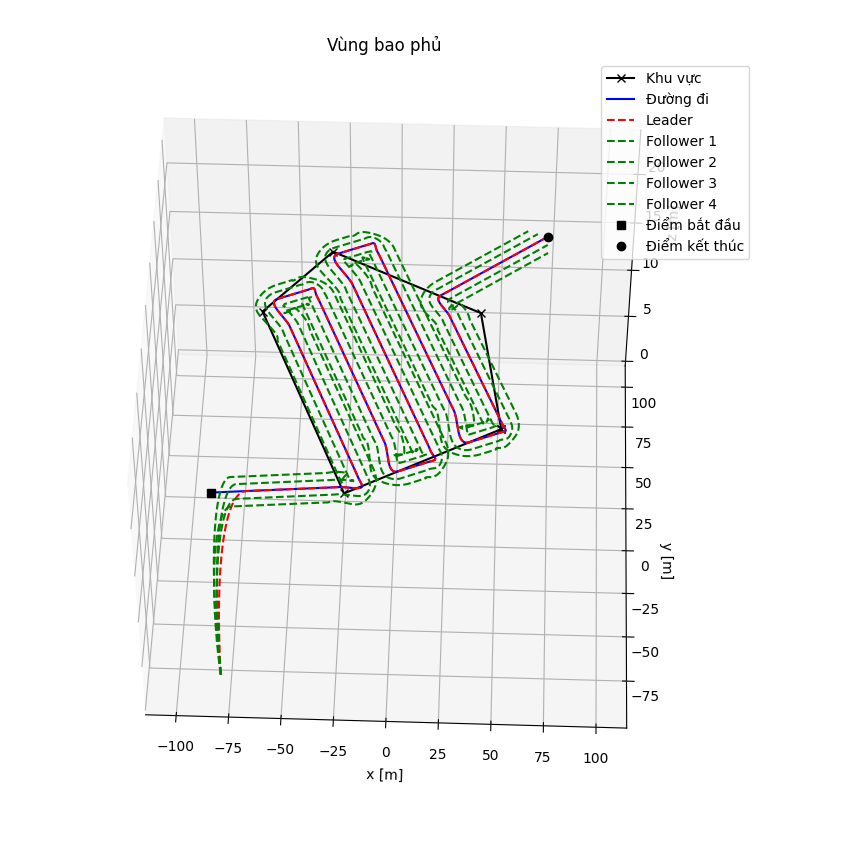
\includegraphics[width=\textwidth]{chapter5/image/coverage1.png}
    \caption{}
    \label{fig:1}
    \end{subfigure}
    %\hspace{-0.5cm}
    \begin{subfigure}[b]{0.8\textwidth}
    \centering
    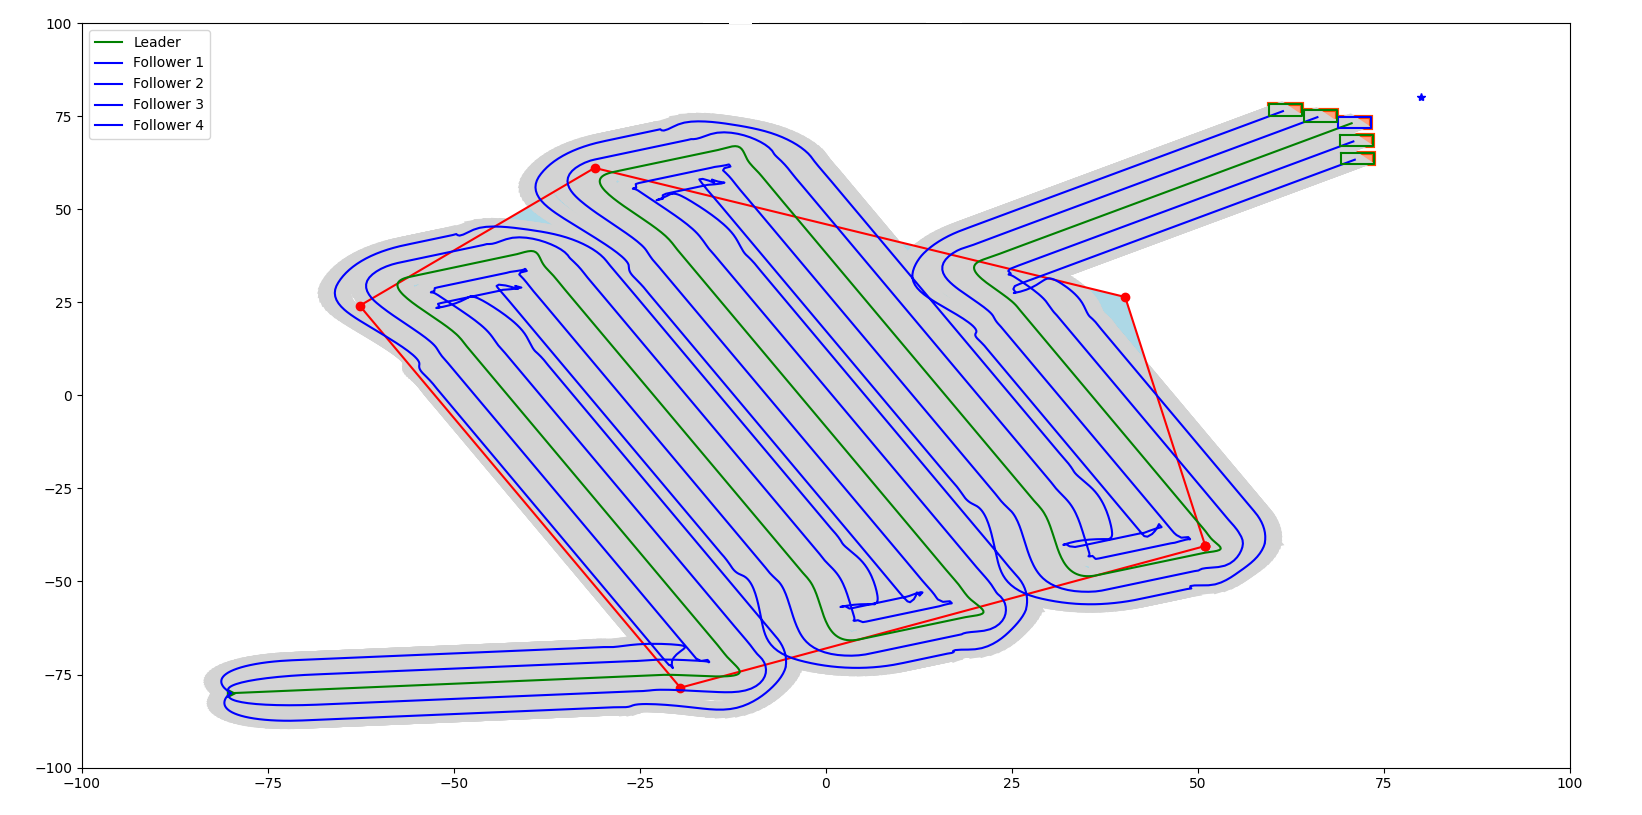
\includegraphics[width=\textwidth]{chapter5/image/coverage.png}
    \caption{}
    \label{fig:2}
    \end{subfigure}
    \caption{Phạm vi bao phủ đội hình chữ V}
    \label{fig:coverarea5Robot}
\end{figure}

\begin{figure}
\centering
    %\hspace{-0.5cm}
    \begin{subfigure}[b]{0.8\textwidth}
    \centering
    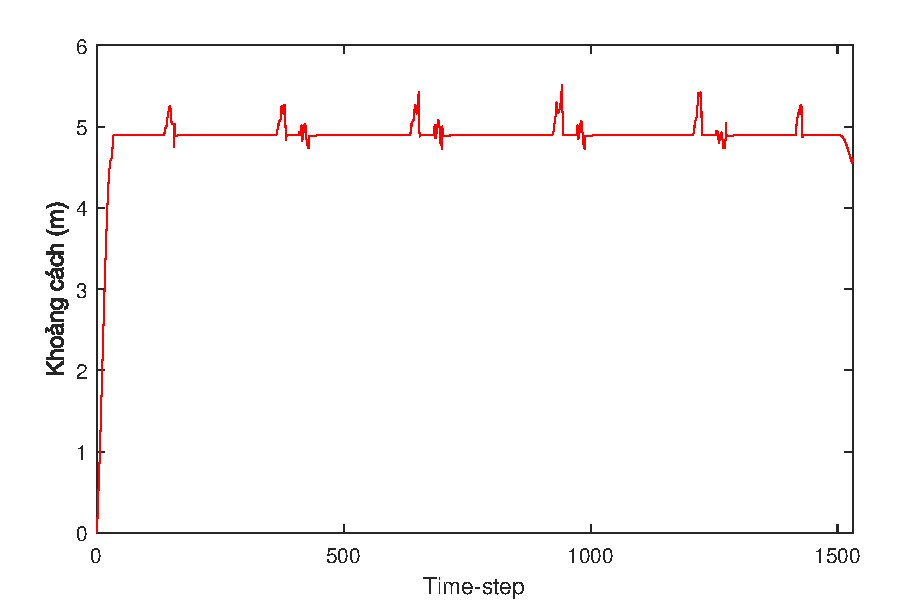
\includegraphics[width=\textwidth]{chapter5/image/Median_Dis.pdf}
    \caption{Khoảng cách trung vị giữa 2 robot liên tiếp}
    \label{fig:Distance5Robot}
    \end{subfigure}
    %\hspace{-0.5cm}
    \begin{subfigure}[b]{0.8\textwidth}
    \centering
    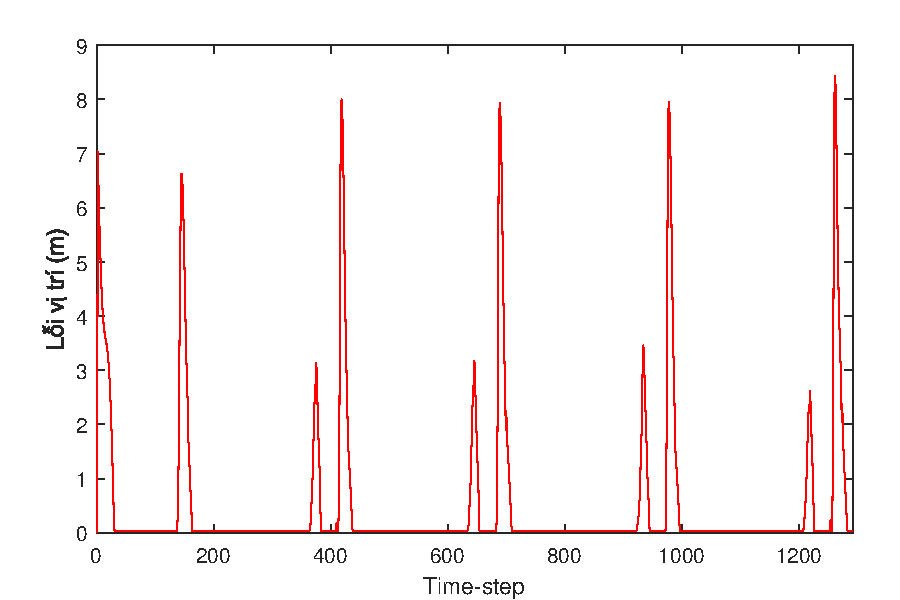
\includegraphics[width=\textwidth]{chapter5/image/Median_Err.pdf}
    \caption{Trung vị về sai số vị trí vị trí follower và các điểm virtual target}
    \label{fig:err5Robot}
    \end{subfigure}
    \caption{Kết quả sự ổn định của quá trình di chuyển đội hình chữ V}
    \label{fig:5Ro}
\end{figure}


Đầu tiên, đầu vào sẽ là khu vực cần được khảo sát có dạng hình polygon ngũ giác. Thuật toán sẽ tiến hành xây dựng và lập đường đi bao phủ cho Leader. Từ đó, quỹ đạo của Leader được hình thành. Trong quá trình di chuyển, Leader sẽ tạo ra cấu trúc ảo có dạng hình chữ V để các Followers có thể di chuyển và bám theo quỹ đạo . Phần này sẽ tiến hành thực hiện một thử nghiệm mô phỏng thể hiện thông qua Hình.\ref{fig:coverarea5Robot}. Trong đó, các đường màu đen là vùng giới hạn của khu vực quan tâm, đường màu đỏ là quãng đường được xây dựng dành riêng cho Leader. Các đường màu xanh lá cây thể hiện được quỹ đạo của 4 robot Followers bám theo để tạo thành cấu trúc hình chữ V \footnote{Đội hình chữ V với 5 Robots \url{https://youtu.be/A5u8xT-GqYQ}}


Kết quả mô phỏng trong Hình.\ref{fig:coverarea5Robot} cho thấy bầy Robot duy trì đội hình chữ V và quét qua toàn bộ vùng khảo sát với tỉ lệ cao là $98.69\%$. Ngoài ra, Hình.\ref{fig:Distance5Robot} chỉ ra rằng mức độ ổn định của đội hình robot trong quá trình di chuyển. Qua đó thấy rằng khi đội hình di chuyển trên đoạn đường thẳng, giá trị trung vị khoảng cách tương đối giữa hai robot liên tiếp luôn được duy trì ở mức ổn định so với tham số đội hình yêu cầu $\ell=4.89 m$, sự giao động chỉ xuất hiện ở các khúc rẽ trong đường đi với độ lệch chuẩn là  $6.44\%$-$12.68\%$. Đối với lỗi vị trí trong Hình \ref{fig:err5Robot}, cũng như trung vị khoảng cách vị trí hiện tại của các followers với các điểm vị trí ảo do leader tạo ra, đường đi thẳng có giá trị trung vị của các vị trí lỗi từ $3.5 m$ đến $8.5m $  khi nó giao động mạnh ở các khúc rẽ của đường zig zac dẫn tới việc robot leader đổi hướng nhanh. Tuy nhiên, nhờ vào hành vi duy trì đội hình được chỉ ra trong chương 2, đội hình chữ V dần dần quay lại trạng thái ổn định. 


Tiếp theo, phần này thực hiện khảo sát thời gian khi bầy robot tiến hành quét qua các khu vực cụ thể. Quá trình mô phỏng sẽ tạo ra ngẫu nhiên 20 vùng khác nhau về diện tích và hình dạng được mô tả trong bảng \ref{tab:Scoverage1}.

\begin{table}[H]
\centering
\caption{Bảng mô tả kích thước các khu vực thử nghiệm}
\label{tab:Scoverage1}
\begin{tabular}{|l|c|c|c|c|c|c|c|}
\hline
\textbf{Map}      & \textit{1}  & \textit{2}  & \textit{3}  & \textit{4}  & \textit{5}  & \textit{6}  & \textit{7}  \\ \hline
\textbf{Area ($m^2$)} & 10789.23    & 8550.85     & 9260.03     & 7966.47     & 8088.73     & 5600.21     & 3408.49  \\ \hline
\textbf{Map}      & \textit{8}  &\textit{9}   & \textit{10} & \textit{11} & \textit{12} & \textit{13} & \textit{14}    \\ \hline
\textbf{Area ($m^2$)}  & 5706.51   & 10224.71    & 9964.78     &9742.46     & 7705.11     & 11979.95    & 24842.79 \\ \hline
\textbf{Map}     & \textit{15} & \textit{16} & \textit{17}   & \textit{18} & \textit{19} & \textit{20}  & - \\ \hline
\textbf{Area ($m^2$)} & 9805.33     & 14419.30  & 10455.92    & 10535.73    & 10846.23    & 14382.34  & - \\ \hline
\end{tabular}
\end{table}

Với 20 vùng bao phủ này, mỗi vùng sẽ được thử nghiệm với số lượng các con robot khác nhau với các mốc 3, 5, 7. Như trên hình \ref{fig:3r},\ref{fig:5r},\ref{fig:7r}:

\begin{figure}[H]
    \centering
    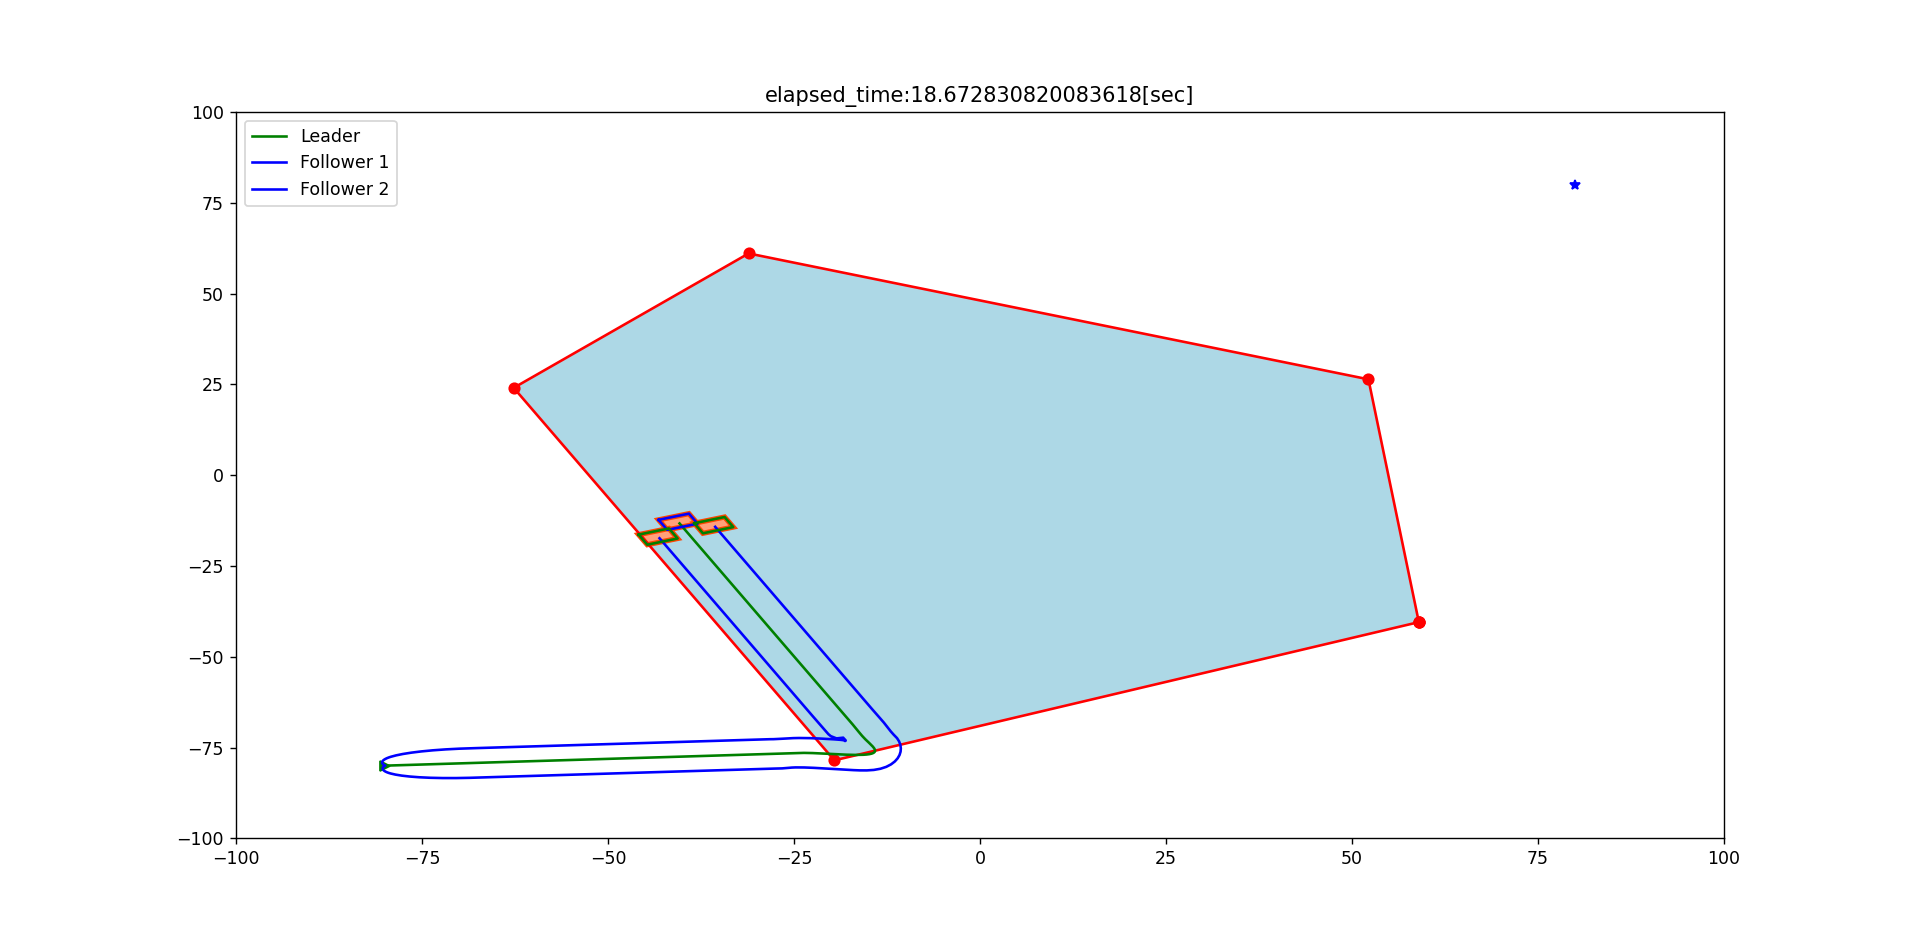
\includegraphics[width=0.8\textwidth]{chapter5/image/3robot.png}
    \caption{Mô phỏng quá trình 3 robot thực hiện quá trình bao phủ}
    \label{fig:3r}
\end{figure}

\begin{figure}[H]
    \centering
    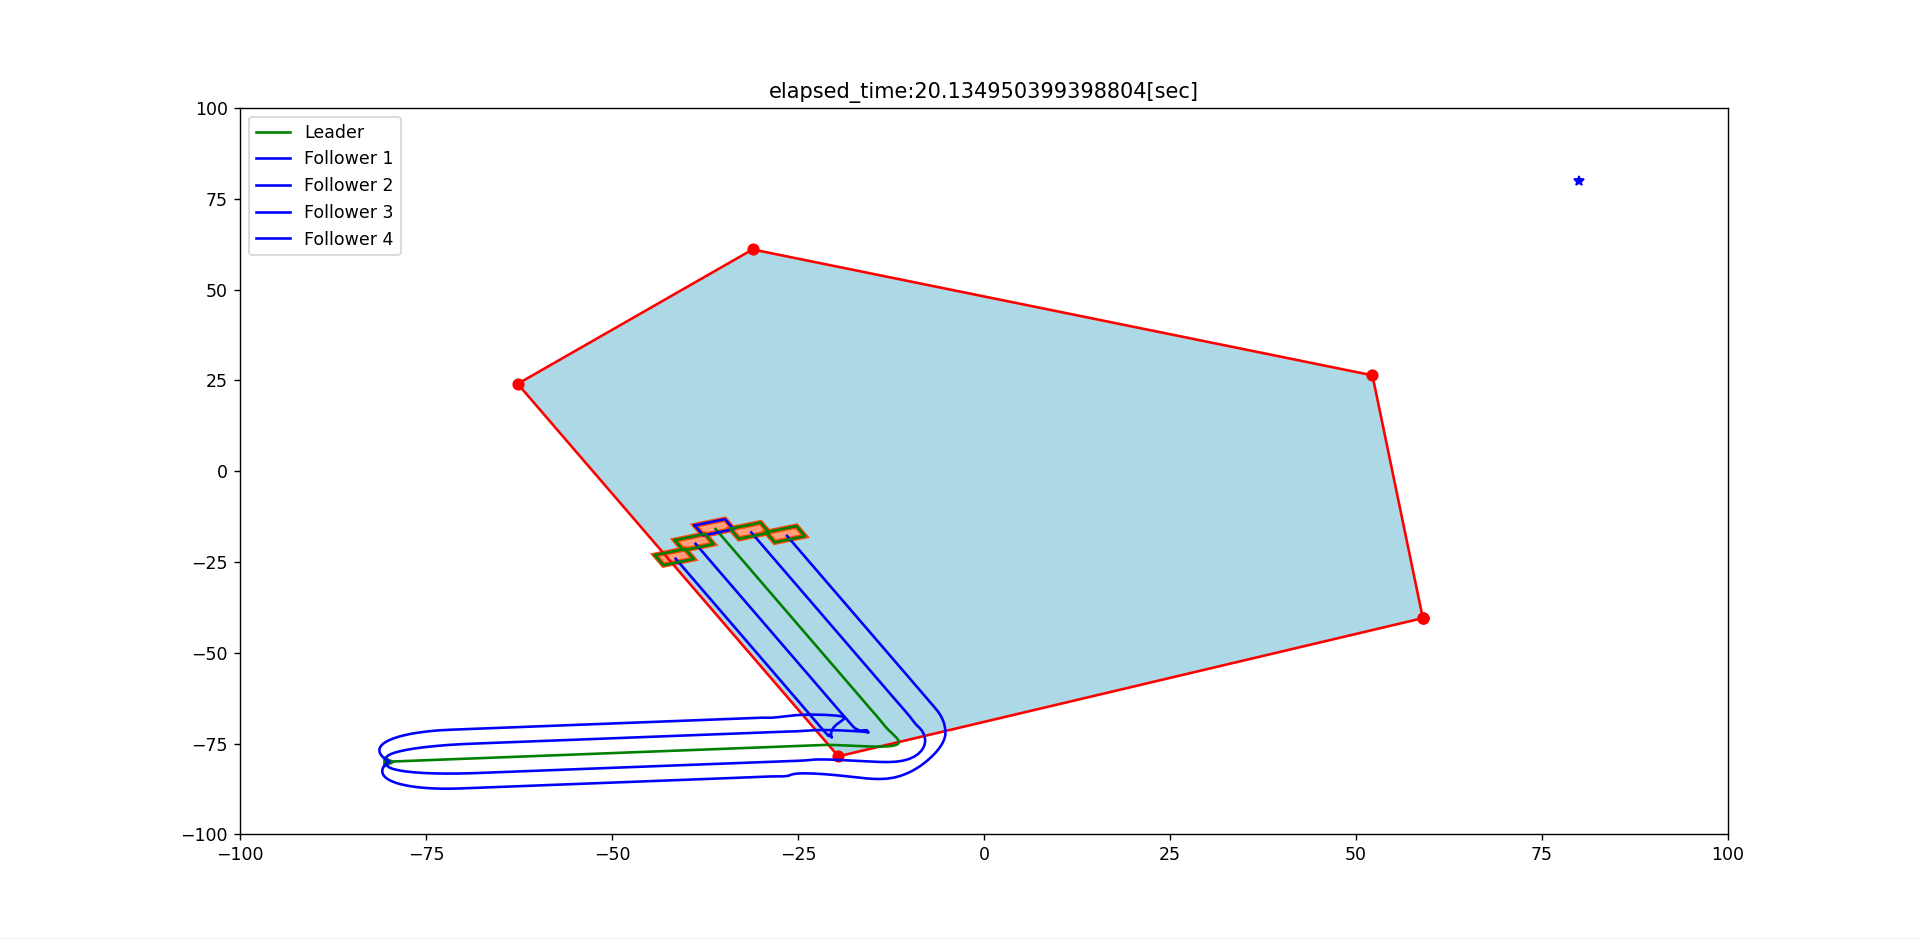
\includegraphics[width=0.8\textwidth]{chapter5/image/5robot.png}
    \caption{Mô phỏng quá trình 5 robot thực hiện quá trình bao phủ}
    \label{fig:5r}
\end{figure}

\begin{figure}[H]
    \centering
    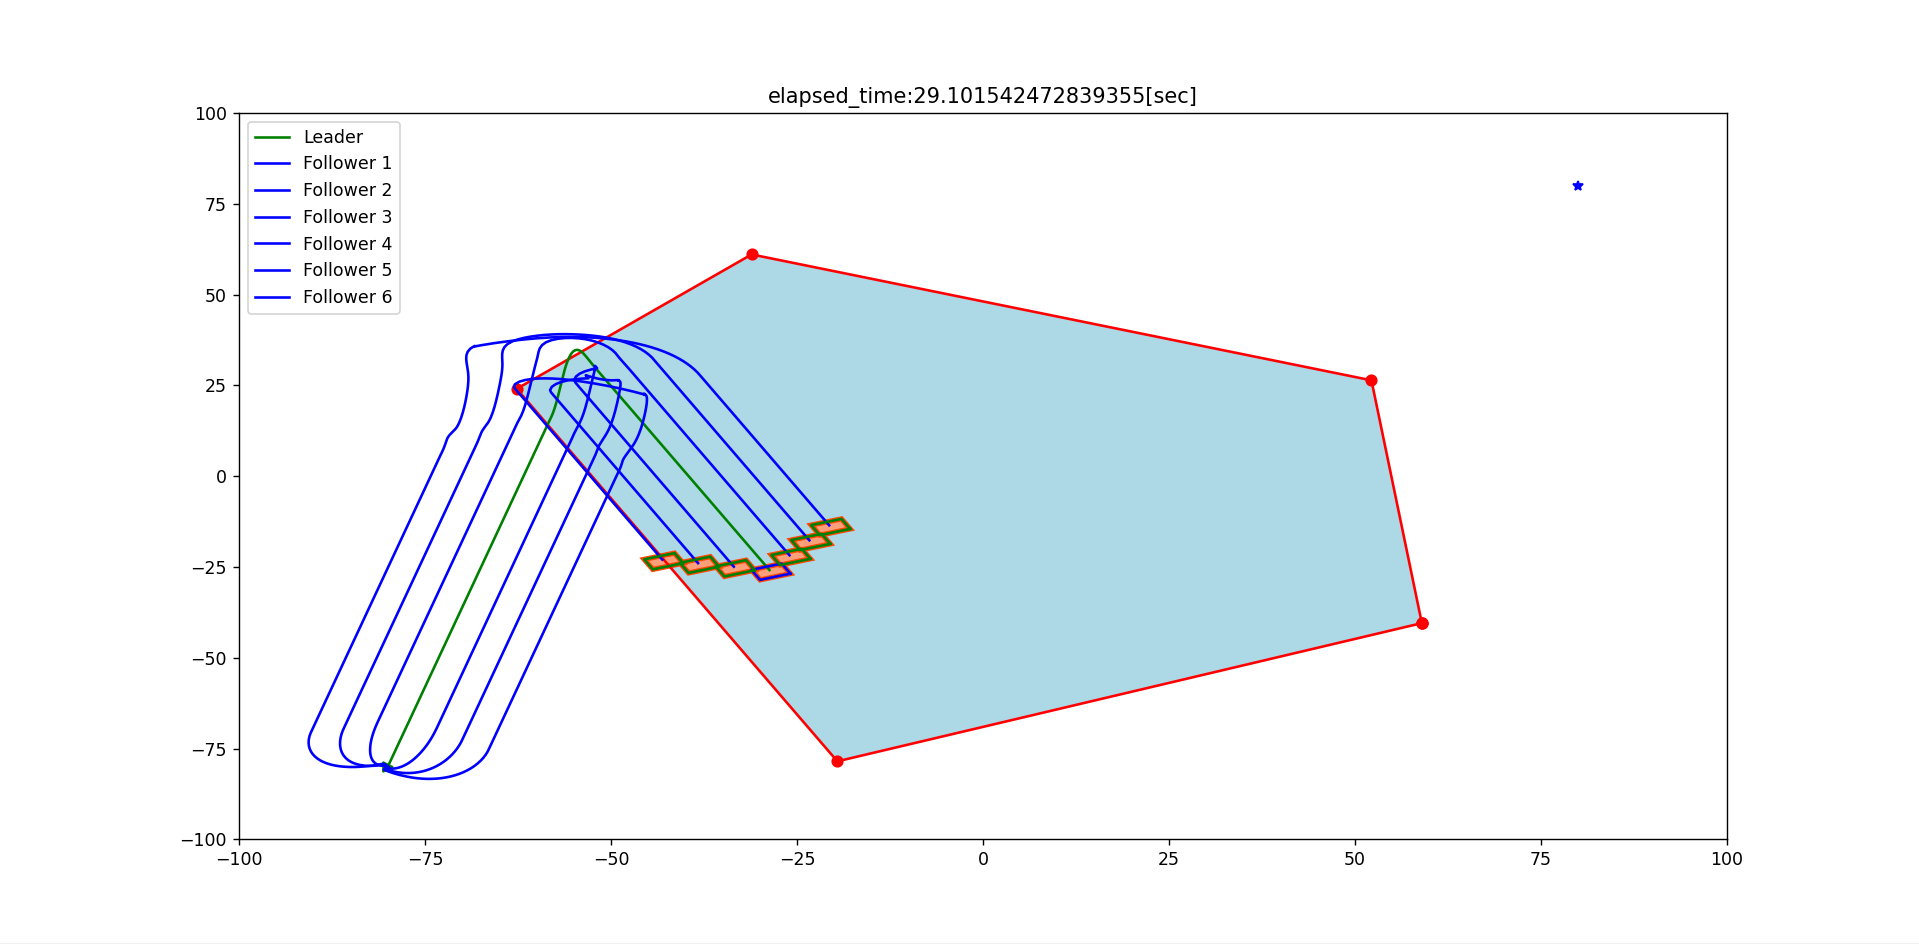
\includegraphics[width=0.8\textwidth]{chapter5/image/7robot.png}
    \caption{Mô phỏng quá trình 7 robot thực hiện quá trình bao phủ}
    \label{fig:7r}
\end{figure}

Cùng với đó, các robot sẽ được đưa vào thử nghiệm các trên 3 giải thuật khác nhau bao gồm: Đường đi bao phủ tốt nhất(Op-RCPP) được mô tả trong phần \ref{sec:Oppath}, đường đi bao phủ với nhiều khúc quay nhất(nonOp-RCPP)(đây là thuật toán tương tự như op-RCPP nhưng sẽ chọn số lượng đường rẽ tối đa thay vì chọn số lượng đường rẽ tối thiểu), và thuật toán lập đường đi bao phủ dựa trên chia lưới(grid-base coverage path planning) trong bài \cite{nam2016approach} với mục tiêu so sánh. Trong mỗi kịch bản, vị trí xuất phát ban đầu của Robot đều được giữ cố định tại điểm có toạ độ: PS = $(-80;-80;0)$, và vị trí kết thúc hành trình có toạ độ là : PE = $(80;80;0)$. Vì vậy sẽ có tổng cộng là 180 kịch bản được mô phỏng để lấy kết quả.

\begin{figure}[h!]
    \centering
    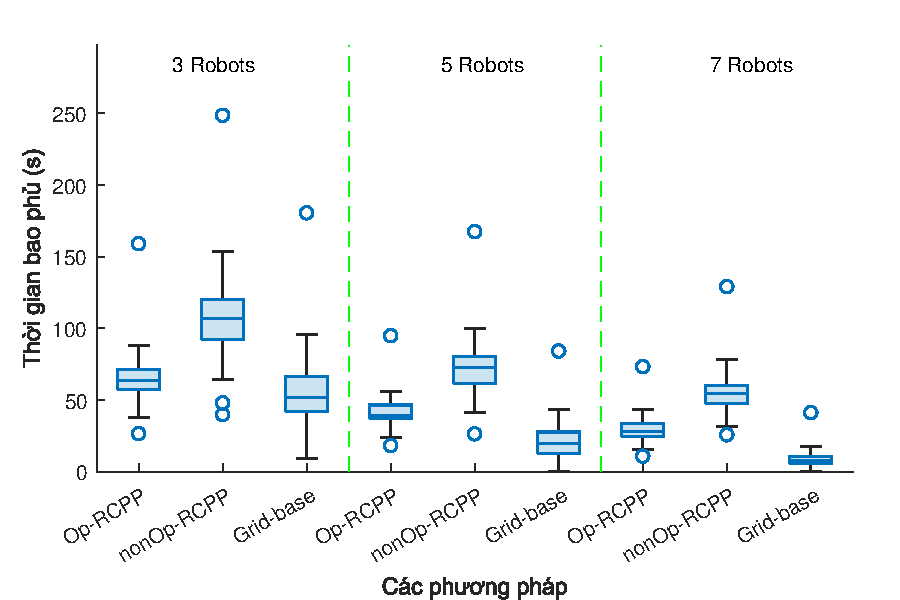
\includegraphics[width=0.8\textwidth]{chapter5/image/CoverageTime.pdf}
    \caption{Thời gian bao phủ với đội hình robot chữ V}
    \label{fig:cov}
\end{figure}

Dựa vào kết quả thu được hình \ref{fig:cov}, có thể thấy được rằng sử dụng thuật toán đường đi tối ưu (Op-RCPP) sẽ thu được kết quả tốt hơn về mặt thời gian bay cũng đồng nghĩa với việc giúp tối ưu về mặt năng lượng khi di chuyển mà vẫn đạt được mục đích bao phủ gần như tuyệt đối. Tuy nhiên khi so sánh với thuật toán không tối ưu(nonOp-RCPP), thuật toán tối ưu đường đi(Op-RCPP) thì sẽ mang lại khả năng di chuyển nhanh hơn gấp $1.8$ lần nhưng độ độ bao phủ lại ít hơn $0.3\% - 8\%$. Điều này xảy ra là bởi vì thuật toán không tối ưu sẽ lựa chọn hướng di chuyển có nhiều góc quay hơn nên sẽ có thể bao phủ tốt hơn tuy vậy thời gian cũng tăng lên đáng kể. 


Đối với thuật toán lập đường đi bao phủ dựa trên chia lưới(Grid-base), trước khi tiến hành khảo sát, do thuật toán còn phụ thuộc vào việc chia độ rộng của lưới hay là độ lớn của độ rộng sải cánh $dx$ của đội hình chữ V, nên sẽ để lộ ra các vùng viền bao quanh bản đồ không thể quét qua làm giảm độ bao phủ, độ bao phủ chỉ tập trung vào vùng trung tâm. Với kích thước của $dx$ càng lớn thì phần không được che phủ càng nhiều. Tuy nhiên thời gian di chuyển sẽ có thể nhanh hơn thuật toán tối ưu đường đi, mặc dù vậy thuật toán này lại có một yếu điểm là trong một số vùng diện tích quá nhỏ không đáp ứng đủ độ rộng sải cánh của đội hình bay dẫn đến trường hợp không thể chia được ô nên thuật toán không thể hoạt động dẫn việc không tạo được đường đi bao phủ. Như vậy thuật toán tối ưu đường đi mang lại kết quả khả quan nhất về mặt thời gian bay bao phủ chỉ phù hợp cho một con robot di chuyển, bao phủ.

 Ngoài ra, khi tăng số lượng robots trong đội hình, thời gian bay giảm. Đặc biệt là trong phương pháp tối ưu đường đi bao phủ, thời gian bay của đội hình chữ V với 5 hoặc 7 robots xấp xỉ giảm $38.84\%$ và $55.58\%$ so với việc đội hình có 3 robots. Nguyên nhân là do khi số lượng robots tăng, sự bao phủ của bầy robot tăng dẫn đến số đường đi giảm.

\begin{figure}[H]
    \centering
    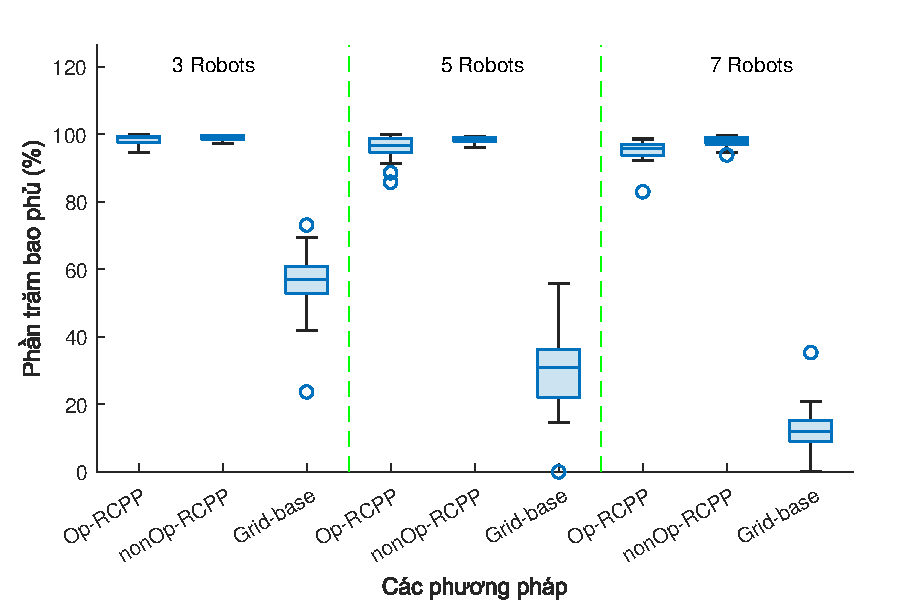
\includegraphics[width=0.8\textwidth]{chapter5/image/CoveragePer.pdf}
    \caption{Tỷ lệ bao phủ với đội hình robot chữ V}
    \label{fig:covPer}
\end{figure}

Kết quả thu được trong Hình.\ref{fig:covPer} cho thấy tỉ lệ che phủ của đội hình Robot chữ V với cả 2 thuật toán bao phủ đường đi (Op-RCPP và nonOp-RCPP) đều đạt được ở mức cao trên $90\%$ đi xấp xỉ đạt được lần lượt là $98.94\%$, $96.80\%$, và $95.66\%$ với từng trường hợp dùng 3, 5, 7 robots. Tuy nonOp-RCPP có vẻ nhỉnh hơn một chút so với Op-RCPP do có nhiều hơn đường đi so với Op-RCPP. Nhưng xét về mặt kinh tế thì để đánh đổi việc bao phủ ít hơn vài $\%$ so với việc tốn nhiều thời gian và nhiên liệu hơn thì có lẽ là không cần thiết. 
Ngoài ra, khi sử dụng đội hình vào trong thuật toán bao phủ dạng lưới(Grid-base), tỉ lệ quét chỉ đạt khoảng $56.88\%$, $30.96\%$, $12.075\%$ tương ứng với đội hình sử dụng 3,5,7 Robots cho thấy sự giảm mạnh so với việc sử dụng Op-RCPP, xấp xỉ lần lượt là $42.07\%$, $65.83\%$, $83.59\%$. Điều này xảy ra bởi vì khi số lượng robot tăng lên đồng nghĩa với việc diện tích bao phủ của bầy tăng lên tức là $dx$ tăng lên. Dó đó đã tác động trực tiếp đến yếu điểm của thuật toán này.


Thí nghiệm cuối cùng sẽ đánh giá quá trình bao phủ của bầy robot khi gặp vật cản. Bài toán này chỉ biết đầu vào là khu vực quan tâm còn không biết thêm thông tin gì về vật cản. Do đó, các robot trong quá trình di chuyển phải tự xác định được vật cản và vượt quá được nó nhờ hành vi tránh vật cản được đưa ra ở Chương 2. Các vật cản có hình dạng như một hình trụ dài hình tròn như ở Hình \ref{fig:obs3d}. Thí nghiệm này được thử nghiệm trên đội hình 5 robot. Kết quả được trình bày bên dưới: 
\begin{figure}[H]
\centering
    %\hspace{-0.5cm}
    \begin{subfigure}[b]{0.48\textwidth}
    \centering
    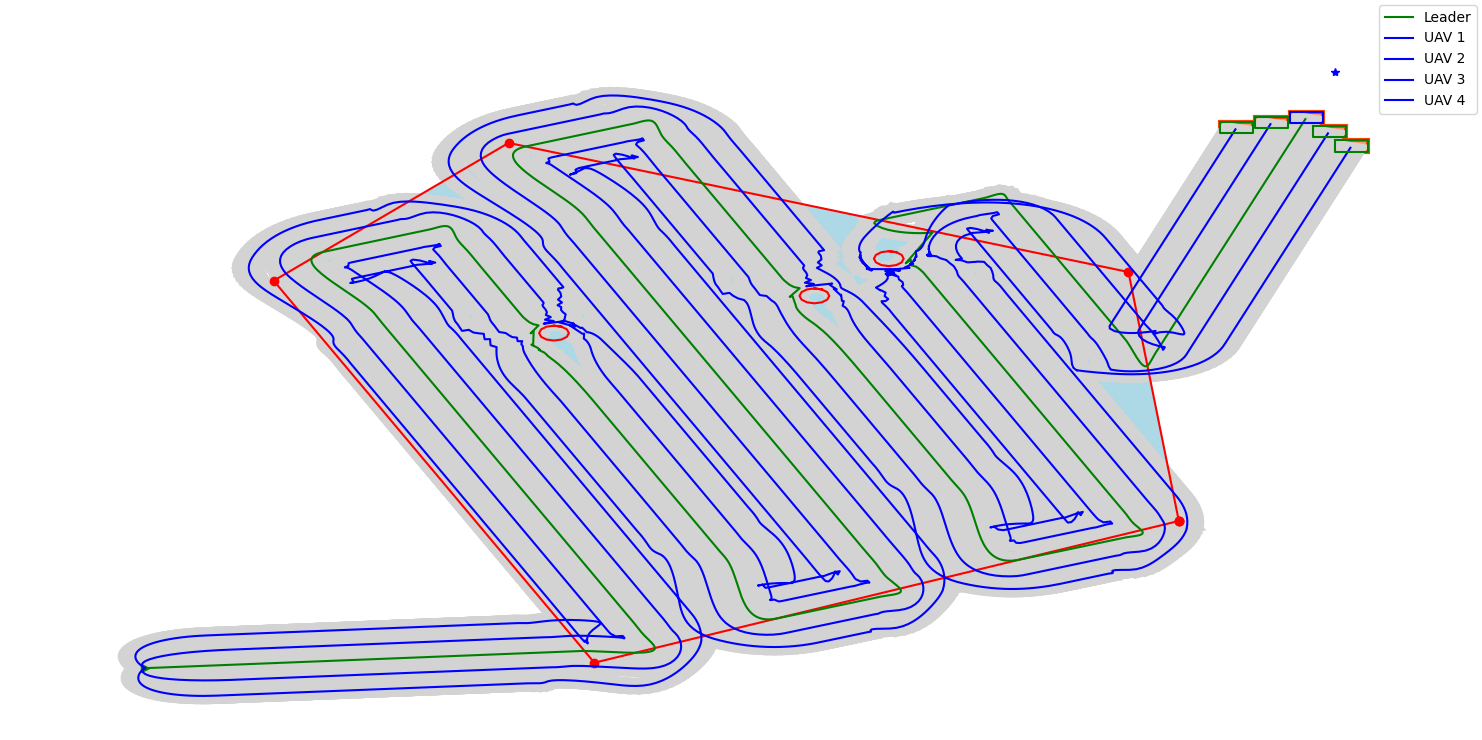
\includegraphics[width=\textwidth]{chapter5/image/obs.png}
    \caption{}
    \label{fig:obs}
    \end{subfigure}
    %\hspace{-0.5cm}
    \begin{subfigure}[b]{0.49\textwidth}
    \centering 
    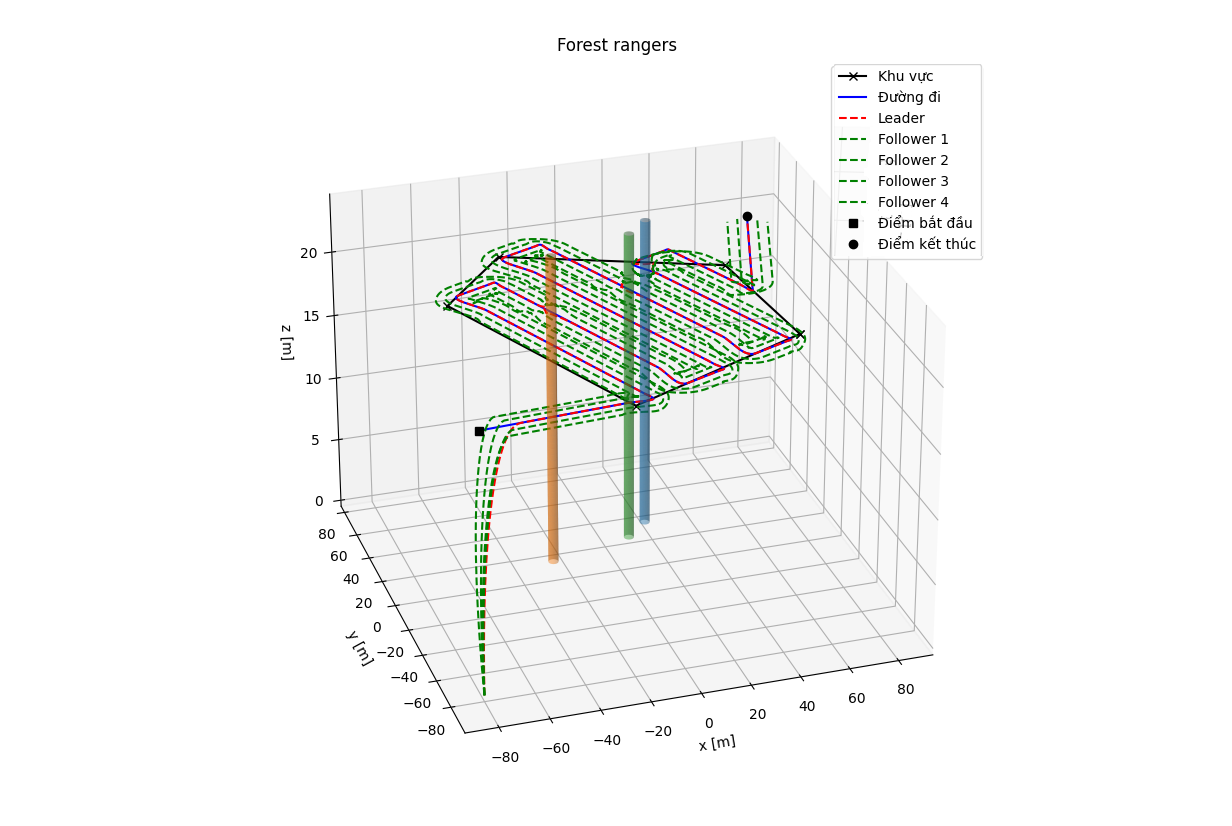
\includegraphics[width=\textwidth]{chapter5/image/obs3d.png}
    \caption{}
    \label{fig:obs3d}
    \end{subfigure}
    \caption{Quá trình di chuyển tránh chướng ngại vật của đội hình chữ V }
    \label{fig:5Robots}
\end{figure}

\begin{figure}[H]
    \centering
    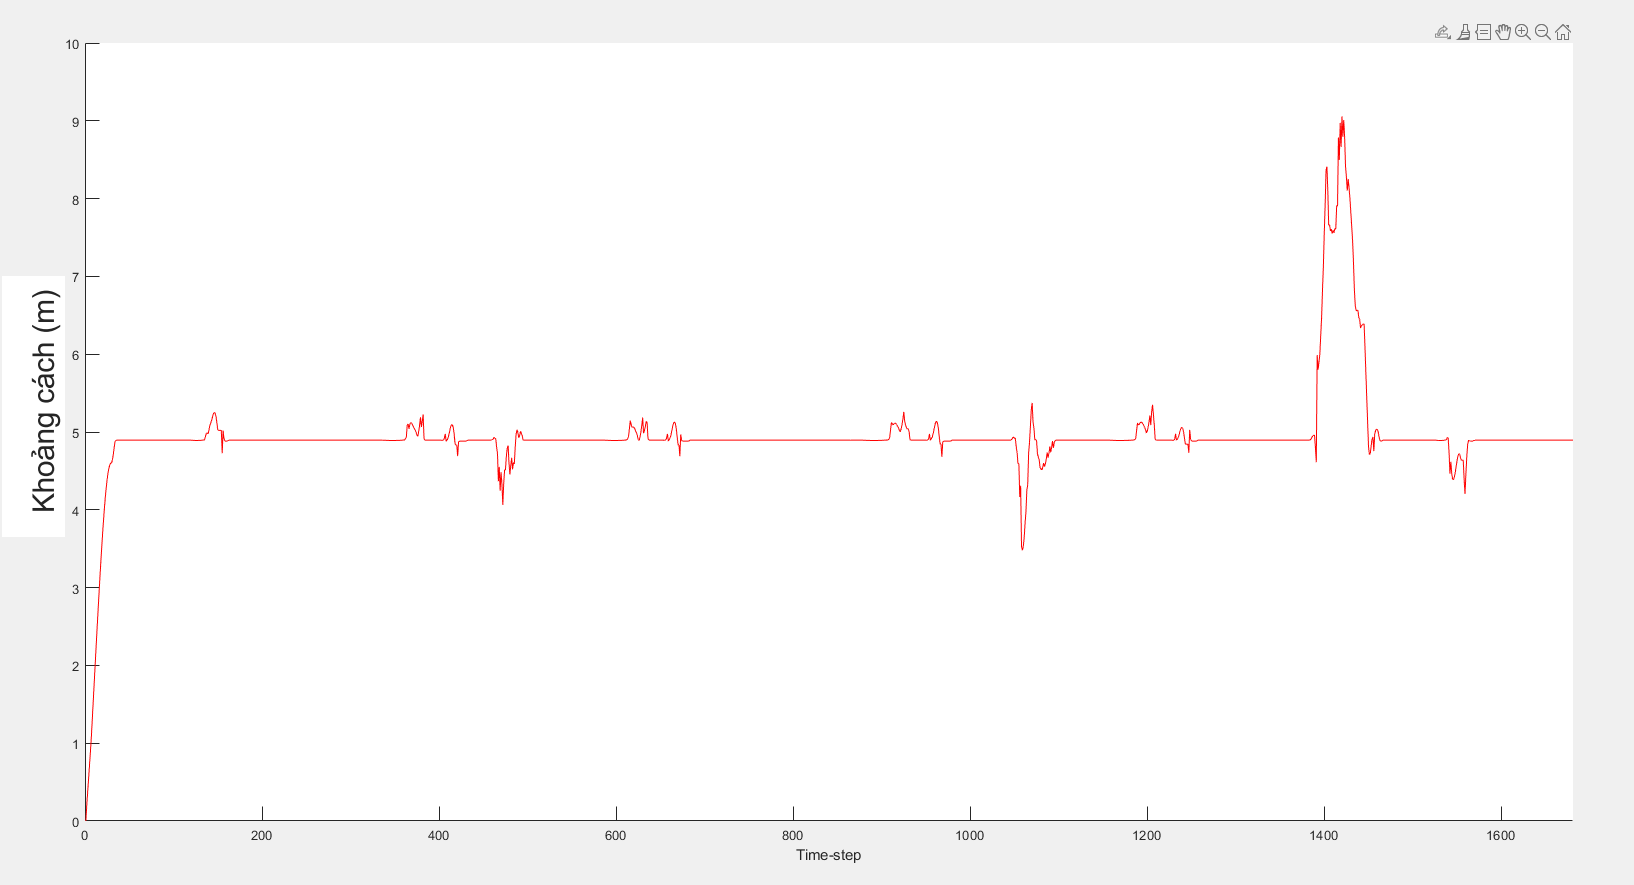
\includegraphics[width=0.8\textwidth]{chapter5/image/poserrobs.png}
    \caption{Khoảng cách trung vị giữa 2 con robot liên tiếp}
    \label{fig:poserrobs}
\end{figure}
Hình \ref{fig:obs} cho thấy được quỹ đạo của các robot trong quá trình di chuyển gặp chướng ngại vật. Các robot đã chủ động tránh vật cản trên đường đi của chúng. Tuy nhiên điều đó đã gây ra sự xáo trộn trong đội hình đặc biệt là khi vật cản ở ngay góc cua sẽ gây ra sự đột biến lớn trong quỹ đạo di chuyển của Leader. Điều này càng được chỉ ra rõ hơn ở trong Hình \ref{fig:poserrobs} khi tránh vật cản, thì khoảng cách trung vị giữa 2 robot liên tiếp không còn được giữ ổn định nữa. Lúc này đã gây ra sự xáo trộn ở trong đội hình. Đặc biệt khi tránh chướng ngại vật thứ 3 ở ngay khúc cua, leader thực sự đã lệch một khoảng cách rất lớn so với quỹ đạo đưa ra. Tuy nhiên nhờ có hành vi giữ đội hình mà đội hình di chuyển dần dần ổn định trở lại và tiếp tục quét các vùng còn lại. Ngoài ra Hình \ref{fig:obs} cũng cho thấy khi quét qua chướng ngại vật thì một phần vùng xung quanh chướng ngại vật không thể bị quét qua, làm giảm hiệu suất bao phủ xuống 91.88$\%$. Tuy nhiên điều này có thể chấp nhận được vì, robot bắt buộc phải thực hiện hành vi tránh vật cản để không gây ảnh hưởng đến đội hình.

Tổng kết, thuật toán tối ưu đường đi bao phủ được đề xuất đã đạt kết quả cao trong cả tỉ lệ quét bao phủ và thời gian bay. Việc sử dụng Op-RCPP để thiết kế đường đi bao phủ khi dùng với nhiều robot thì phù hợp hơn sử dụng phương pháp chia lưới.